% Preamble
% Global
\documentclass[
    parskip=full,
    a4paper
]{scrartcl}
\usepackage{blindtext}
\usepackage[utf8]{inputenc}
\usepackage{etoolbox}

\usepackage{hyperref}
\hypersetup{
    colorlinks,
    citecolor=black,
    filecolor=black,
    linkcolor=black,
    urlcolor=black
}

% Graphics
\usepackage{pdfpages}
\usepackage{graphicx}
\usepackage{xcolor}
\usepackage[many]{tcolorbox}
\usepackage{etoolbox}

% Chars https://tex.stackexchange.com/questions/42619/x-mark-to-match-checkmark
\usepackage{amssymb}% http://ctan.org/pkg/amssymb
\usepackage{pifont}% http://ctan.org/pkg/pifont
\newcommand{\cmark}{\ding{51}}%
\newcommand{\xmark}{\ding{55}}%

% Lists
\usepackage{enumitem}
\setlist{nosep} % or \setlist{noitemsep} to leave space around whole list

% Tables & figures
\usepackage{multirow}
\usepackage{array}
\newcolumntype{$}{>{\global\let\currentrowstyle\relax}}
\newcolumntype{^}{>{\currentrowstyle}}
\newcommand{\rowstyle}[1]{\gdef\currentrowstyle{#1}%
  #1\ignorespaces
}

% Layout
\usepackage[margin=1.25in]{geometry}
% \hoffset .25in
\usepackage{setspace}
\usepackage[utf8]{inputenc}
\usepackage[english]{babel}
\setstretch{1.3}
% \setlength{\parindent}{0em}
% \setlength{\parskip}{1em}

% Inline-code
\usepackage[outputdir=./_build]{minted}
\definecolor{dhscodebg}{rgb}{0.01,0.199,0.1}
\setminted{
    breaksymbolleft=,
    fontsize=\footnotesize,
    baselinestretch=1.1,
    % bgcolor=dhscodebg,
    % rulecolor=\color{gray!40},
    % framesep=\fboxsep,
    % frame=single,
    % framesep=10pt
    % framerule=2pt,
    xleftmargin=2.5em,
    linenos,
    breaklines,
    tabsize=4
}
\usemintedstyle{tango}
\BeforeBeginEnvironment{minted}
{\begin{tcolorbox}[
            breakable,
            boxrule=0.2pt,
            colback=gray!40,
            % toprule=1pt,
            % rule=1pt,
            arc=0pt
        ]}\AfterEndEnvironment{minted}{\end{tcolorbox}}

% Bibliography
\usepackage{natbib}
\usepackage{bibentry}
\nobibliography*

% Title
\title{Entity aggregation via MapReduce in CouchDB}
\author{Zach Smith}
\date{\today}

% Document
\begin{document}

% Title page
\maketitle
\thispagestyle{empty}

% Abstract
\begin{abstract}
    CouchDB allows users to define \textit{MapReduce} functions to calculate indexed views of databases with the aim of fast data retrieval. These views are stored as as B+trees and are cached to disk storage. Dispersed index calculation makes CouchDB suitable as a tool for handling large amounts of data via large clusters of commodity hardware with the caveat that querying such a data store is limited according to CouchDB's implementation of \textit{MapReduce}. Indexed output from disparate entities is straightforward in CouchDB as is shown via the aggregation of several different entities involving students at the University of Cape Town. However, joining data in CouchDB is limited for two reasons: 1) The indexing engine only works if reduced results are substantially smaller than the input (aggregations work well), and 2) it was found that for practical purposes using reduction is limited to what is achievable with CouchDB's built-in \textit{\_sum}, \textit{\_count}, and \textit{\_stats} reduce functions due to performance degradation when specifying custom logic (although the query API allows for this). Such a limitation, in turn, limits the extent to which entities can be grouped according to input types required by the built-in reduce functions. As such, certain join operations (i.e. queries that require SQL-like \textit{GROUP BY} phrases) are not easily implemented using CouchDB \textit{MapReduce} indexes.
\end{abstract}
\newpage

%  TOC
\tableofcontents
\newpage

% Content
\section{Introduction}
Insights into student grades, class/online participation, material engagement, demographic information and more allows for data-driven feedback on different approaches to learning and teaching. As such, exploring the plethora of data that learning management software such as UCT's Sakai platform collects has the potential to greatly improve the educational experience through data-mining. Intrinsic to this process is the concept of data-storage and retrieval - a topic that is becoming ever more important as the amount of data collected increases exponentially. As alternatives to traditional relational-orientated databases are become preferred software for housing large data stores in many cases, a mentality shift from data retrieval via the SQL (structured queried language) standard is required. Although many new NoSQL databases due implement a version of the SQL standard for querying, many do not. An alternative paradigm, and the subject of this project is \textit{MapReduce}, a framework for data querying that allows for infinitely dispersed data storage and processing, and by association, infinite possibilities in the world of data-mining.

\subsection{Project Significance}
An investigation of CouchDB's \textit{MapReduce} implementation in terms of how it handles querying of relational entities (and how) is the first step in assessing the databases suitability as a store for large amounts of data for the purposes of mining in the context of educational management systems. CouchDB is a new technology that embodies much of the NoSQL trend; a schema-less data model, MapReduce queries, open-source code-base and suitability for distribution over commodity hardware. This analysis will provide information for consideration when designing data-mining architectures of the future - be that in support of educational data-mining, general database usage, availability, etc. If CouchDB were a suitable technology for implementation within large-scale data architectures, that nature of a highly-available data store with mobile, browser and server implementations raises some interesting possibilities in terms of data access within the South African context - where data is expensive and there are still areas where university students have slow internet access.
\subsection{Motivation \& Aim}
The Couchbase project \cite{couchbaseWhitePaper} mentions that in recent times, much of that data being produced on a day-to-day basis is semi-structured or unstructured due to the diversity of the kind of devices and users that are using data-collecting devices. RDBMSs seem ungainly in this scenario with their strictly defined data models making handling unstructured data cumbersome and expensive in terms of implementation time, and complex in terms of architecture and design. Additionally, systems like Oracle, DB2, SQL Server, MySQL and others scale more easily vertically than they do horizontally \cite{couchbaseWhitePaper}, which is comparatively limiting and expensive. Unlike RDMSs, NoSQL databases with their unstructured data models allow for easy expansion beyond single servers to many, many servers fairly easily and allow for a more agile approach to data modeling since data does not have to be statically modeled, and a model can changed very easily as a system evolves. Such is the motivation for rendering a data-analysis on student grade/event (semistructured) data with a NoSQL database (in this case CouchDB). In general, there has been substantial uptake of NoSQL data solutions such as CouchDB, Couchbase, Mongo, Cassandra and other solutions at the expense of established RDBMSs.

CouchDB is a scalable JSON storage that allows for database sharding (clustering features were added to CouchDB 2.0 released in 2016 with the merge of IBM's Cloudant code \cite{couchdb2.0}) across multiple commodity servers very easily. Theoretically, CouchDB as a data store is suitable for storing an unlimited amount of unstructured data at affordable infrastructure costs. It is also substantially cheaper to license than many RDBMSs since it is open source and available for free. This project looks to assess CouchDB in terms of being a viable alternative to working with data where SQL operations (JOINS in particular) are a common business requirement.

CouchDB supports additional features that make it suitable for usage in a modern, ultra-connected world; an HTTP API. Unlike other databases with inconstant and undocumented protocols for communication between the database server and clients, CouchDB's HTTP interface allows for easier data accessibility. Both in the variety of ways data can be accessed (directly within a browser for example) as well as the ease of accessing data (via URLs either written by hand or via server/browser \textit{JavaScript}). Such features make CouchDB a suitable tool moving into the information-orientated society of the future where an 'agile' approach to data storage becomes the norm within an ever-more connected (in terms databases) world. The HTTP interface also allows for the idea of 'CouchApps', where HTML is served directly from documents stored in the database to browsers. This was originally a CouchDB draw-card for many as seen in this open email exchange \cite{googleCon2017} by Apache Foundation members. However, this same exchange shows (unfortunately) that the "CouchApp" feature of CouchDB is unlikely to survive future releases due to lack of interest in contributing to this feature.

In short, CouchDB is innovate as a database and allows for innovative system as a result. It would be useful for a better idea on the feasibility of it's usage for different use cases. This project aims to look at feasibility of querying data in CouchDB compared to similar queries in a SQL environment.
\subsection{Related work}
Falling under the umbrella category of \textit{Educational Data Mining} (EDM), much work has been done with the intent of modeling student performance as dependent on certain markers such as attendance, assignment and test grades, high school marks, demographic data, etc. Different means of model generation have been discussed by the EDM community such as predictive analysis via decision tree generation as recently done by Honors-level students at UCT \cite{Balestra2017,casper2017} and several other researchers \cite{Qasem20016,Dimitris,zebun2005,Mierle:2005} with varying results. Many other models have been applied within the field of EDM as discussed in a review of EDM up to 2009 by (\cite{bakerEdMiningSummary}).

Although these studies discuss analysis-frameworks at length, very little work has been done on the underlying data stores that form a basis of such analysis. As such, it appears that the work done so far looks to research feasible models in terms of accuracy and implementation rather than feasible means of implementing such mining techniques. Where \textit{Extraction, Transformation, and Loading} (ETL) processes have been discussed with regards to data preparation, SQL is used but without much discussion as to the implementation of the underlying relational data stores (\cite{Balestra2017,casper2017,Mierle:2005}). No attempts have been made to use newer and less conventional NoSQL stores such as CouchDB despite that benefit that such data stores provide in terms of the unique features that these newer data stores offer (\textit{schema-less} entites, easier scaling, lower costs of implementation and licensing, etc.).

\subsubsection*{NoSQL Overview}
Fundamental to the concept of data storage is the implementation of \textit{ACID} constraints - \textit{A}tomicity (transactions either fail or succeed), \textit{C}onsistency (a database's state should always be consistent regardless of transactions), \textit{I}solation (transactions are self-contained) and \textit{D}urability (data is persisted reliably). Such constraints are well understood in RDBMSs and are fundamental to RDBMS usage; that they are often not translatable to NoSQL solutions means that data-handling via a NoSQL data store needs to be approached from a fundamentally different perspective.

Such idioms as \textit{BASE} - \textit{B}asically \textit{A}vailable (data stores are optimized to be available at the expense of consistency), \textit{S}oft state (allowance that state is inconsistent even across a single transaction) \textit{E}ventual consistency (data stores update to become consistent) are provide alternative frameworks to the \textit{ACID} metaphors and are solutions to the trade-offs required as per the \textit{CAP} theorem \cite{GANESHCHANDRA201513}: i.e. that a database represents a trade-off between 3 properties: \textit{consistency}, \textit{availability} and \textit{partition tolerance} with only 2 of the 3 properties fully achievable in a single system. As mentioned by the authors in \cite{GANESHCHANDRA201513}, modern (NoSQL) databases are focused on \textit{available} systems, where data layers are always available to users regardless of consistency (because the alternative is that user interactions fail). Generally (as in the case with CouchDB), availability is achieved via eager replication with some level of consistency applied via the idea of a quorum. CouchDB, when configured to work in sharded clusters with multiple copies of each shards (on different nodes), allows for configuring successful read/writes only when document representation is agreed upon by a set number of nodes. Because of the potential for inconsistency, NoSQL seeks to provide a 'relaxed' viewing model - i.e. \textit{Soft state} views where data representation is not tied to the underlying entities (an entity can be updated whilst being viewed unaware of such changes). That is, sacrificing of \textit{availability} at the expense of \textit{consistency} as per the \textit{cap} theorem; data conflicts, where entities are updated separately and independently of each other are often acceptable in NoSQL databases - particularly in an offline-first approach to data-handling.

Despite moving away from the relational model as provided by RDBMSs, the concept of 'entities' is usually still highly relevant in many NoSQL databases; these database can, as such, be grouped into two categories:

\begin{enumerate}
    \item \textit{aggregate orientated} stores that model data similarly to the relational model but with isolated entity boundaries (\cite{fowlerAggregate}) and
    \item \textit{aggregate ignorant} stores where the concept of entities is fundamentally different (e.g. a graph database such as \textit{Neo4J} where the entities are edges and nodes)
\end{enumerate}

By far, most databases operate within a domain where data is for the most part entity-driven. The family of \textit{aggregate orientated} NoSQL data stores include \textit{key/value} stores such such as Amazon's \textit{Dynamo} database, column based stores such as \textit{Cassandra}, \textit{HBase} and document stores such as \textit{CouchDB}, \textit{Mongo}, etc. As \cite{GANESHCHANDRA201513} points out there are hundreds of NoSQL data stores and a comprehensive categorization of such products is not sensible. Although NoSQL databases are said to be \textit{schema-less}, \cite{ATZENI2016} points out that this is not the case: instead NoSQL allows for inconsistent schema representation across different entity instances due to the nature of aggregations. Such flexibility is at the heart of document stores such as CouchDB and Mongo where loose-schema modeling is one of the properties that makes such technologies suitable for large systems that generate data from inconsistent sources (i.e. a constant 'survey' entity with each instance having different questions). As aggregates, instance-specific \textit{ACID} constraints CAN be implemented by \textit{aggregate oriented} data stores. CouchDB, for example, guarantees atomicity at a document level and optionally when inserting many documents at a time (using the \textit{bulk\_docs} endpoint \cite{bulkDocs}). Despite this, CouchDB doesn't support the idea of multistep transactions in the same was as many RDBMSs do. "Multi-step transactional atomicity" is a key feature for many RDBMSs including \textit{MySQL}, \textit{SQL Server}, etc. and overcoming this limitation is something that is required in order to implement NoSQL databases in traditional RDBMS environments. This is possible, as shown by \cite{Rashmi2017} for CouchDB specifically and NoSQL in general \cite{LOTFY2016133} via implementing \textit{ACID}/transactional properties as bespoke middleware externally to these DBSs. But it would seem this is not an ideal way of replacing RDBMS products due to the complexity and the potential for error that bespoke software, in such an important aspect of business logic as data storage, introduces.

Prior to CouchDB 2.0, middleware was also used for implementing sharding in CouchDB \cite{CORBELLINI20171}. However due to the nature of the CouchDB software itself, indexing such systems would have resulted in additional complications since the indexing engine of CouchDB prior to 2.0 did not allow dispersed calculations. In terms of classifying CouchDB within the NoSQL solutions, it is undoubtedly a document store but with certain characteristics of a \textit{key:value} data store due to the fine grained control users have over index creation on the nature of how those indexes are queried. In such cases, CouchDB mimics \textit{key:vale} database characteristics such as \textit{Redis}, \textit{MemCached}, \textit{Dynamo}, etc. \cite{MAKRIS201694,CORBELLINI20171,GANESHCHANDRA201513}.

The concept of data warehousing is also starting to undergo a shift towards a NoSQL mentality \cite{BICEVSKA2017104}. These authors point out that while very well suited to fact-table representation of structured data, there is still the requirement for handling and storing less structured data as well. Some advantages of turning to unstructured data warehousing technologies include, similarly to the move from structured to less-structured databases in general, easier and more agile development, easier storage of more types of data and as a result, potential for more meaningful and comprehensive data analysis. As \cite{BICEVSKA2017104} mentions, in this regard, NoSQL databases are likely to provide the most value when used in conjunction with traditional RDBMSs.

\subsubsection*{Querying via MapReduce}
In response to dealing with huge amounts of data on a daily basis, authors at Google (Jeffrey Dean and Sanjay Ghemawat) outlined a programming model that abstracted complications associated with distributed computing such as how to parallelize processing, data distribution, fault tolerance, load balancing and execution time \cite{Dean:2008}. This model, known as \textit{MapReduce}, provides programmers a conceptually-simple interface for specifying dispersed data computations succinctly and hides implementation details. The framework relies on an astoundingly simple programming model described by \cite{Dean:2008} as a computation that takes a set of input \textit{key:value} pairs and produces a set of output \textit{key:value} pairs via the following 3 steps:

\begin{enumerate}
    \item A \textit{mapping} stage in which distributed \textit{key:value} pairs are produced from input data as described by a user-defined \textit{map} function
    \item A \textit{grouping} stage where distributed \textit{key:value} output from the mapping stage is collected to common \textit{keys} - i.e. \textit{key:[value, value, value]} datasets
    \item And a \textit{reduce} stage where \textit{values} per key \textit{key} are processed as described by a user-defined \textit{reduce} function
\end{enumerate}

Due to the distributed and isolated nature of \textit{map} and \textit{reduce} tasks, \textit{MapReduce} as an idea is greatly fault tolerant (fault tolerance is implemented via reexecution), which has in turn resulted in the "New Software Stack" as mentioned by \cite{mining2011} - large scale computing clusters built on commodity (cheap) hardware and software that computes in parallel. The "New Software Stack" represents processing ever-greater amounts of data at ever cheaper rates and has spurred information explosion across all manor of software applications.

With the development of the \textit{Hadoop} framework as an open-source alternative to Google's proprietary file system and MapReduce framework, data computations within a MapReduce context have become mainstream. As \cite{chandar2010} discusses in his MSc thesis "Join Algorithms using Map/Reduce" made available by the University of Edinburgh, many companies now utilize this idea including Yahoo, Facebook, Amazon and many others (The Apache Foundation maintains a list of companies that use the Hadoop framework \cite{hadoopPower:2017}).

With increasing update within a data-analysis context, it is fair to say that many of the algorithms required on a day-to-day basis in common data-querying tasks can be implemented via the MapReduce framework including \textit{relational-algebra} operations such as \textit{selection}, \textit{projection} (selection of a subset of attributes from a tuple), \textit{union}, \textit{intersection}, \textit{difference}, \textit{joins} (non-equi joins cannot be implemented via MapReduce), \textit{grouping} and \textit{aggregation} \cite{mining2011}.

As mentioned by \cite{chandar2010} both \textit{Two-Way} and \textit{Multi-Way} joins can be implemented via the MapReduce framework in general, though this is dependent on specific implementations of MapReduce. \textit{Two-Way} joins can be achieved via MapReduce using \textit{Reduce-Side Join}, \textit{Map-side Join}, and \textit{Broadcast Join} algorithms. As the subject of his thesis, \cite{chandar2010} outlines and measures performance for \textit{Multi-Way} joins using \textit{Map-Side Join}, \textit{Reduce-Side One-Shot Join},\textit{Reduce-Side Cascade Join} algorithms. The author found that \textit{Multi-Way} joins were feasible using MapReduce, and that implementation complications of a dispersed system were hidden (as expected) by the Hadoop framework. In other words, \cite{chandar2010} found that relational operations are feasable within dispersed systems running the MapReduce framework.

\section{CouchDB}
\subsection{CouchDB's MapReduce implementation}
CouchDB as a document store doesn't, in itself, provide a means of data-querying. Instead it allows for processing of database file(s) via MapReduce to produce separate files (\textit{Views}) that are derived from a single database. These derived sets of data are structured as B+Trees, as are the initial database files. To this extent, and as pointed out in \cite{couchguide}, CouchDB is effectively a B+tree engine that provides users a means of interacting directly with B+trees via an HTTP API. Via this API a user is able to interact directly with the database B+tree, to which all view files are linked; changes to a database file results in incremental adjustment of the view file via the specified MapReduce functions. So in a sense you don’t 'query' couch. You actually specify a MapReduce task to create a completely separate store of data. And then you can interact with that data (specifically by searching) using the REST API.

In this sense the isolated nature of MapReduce (specifically the implementation in CouchDB) allows eager creation of 'query' output (if you were to consider view-generation as a means of 'querying' CouchDB) across huge, dispersed and highly available query output. Unlike in the traditional sense of 'MapReduce', Couch's reduce engine allows for partial groupings of a key via specifying the concept of 'rereduction' in the contract of the reduce function. More accurately, \textit{map} results are stored as B+ indexes within CouchDB including \textit{reduce} results on internal nodes (see \ref{appendix:slack1}). As mentioned on the original (and no longer maintained) CouchDB Wiki, \textit{map} output is sent the \textit{Reducer} in batches delimited by B+tree boundaries \cite{couchwiki}. Since grouping is done after this step by the \textit{Reducer}, reduce functions must allow for the case that not all values for a key are processed at once or by the same \textit{reduce} function. This allows for dispersed, partial and autonomous view calculation on any CouchDB node.

In terms of how MapReduce is executed in CouchDB, and possibly related to B+tree storage structures as mentioned above, grouping and reducing in CouchDB is handled by a 'master' node for any particular shard. Unlike a traditional implementation of MapReduce where \textit{Map} and \textit{reduce} tasks are executed in parallel, CouchDB spawns a single \textit{couchjs} process per shard (see \ref{appendix:slack3} and \ref{appendix:slack5}) and the map index is calculated sequentially according to a list of database changes as managed by CouchDB (available at the \textit{\_changes} endpoint).

Worth mentioning in the context of couchDB specifically, is the MapReduce engine used. CouchDB ships with an executable "couchjs.exe" - the \textit{javaScript} query-server - coupled with Mozilla's \textit{SpiderMonkey} runtime engine; this query engine is drop-in replaceable, although there is probably no motivation to do so. According to the documentation \cite{builtincouchreduce}, CouchDB has with a couple built-in reduce function - \_sum, \_count, and \_stats that are implemented as functions within the main Erlang process (as distinct from the mapping and reduction being handled by the main process) that perform substantially better than custom reduce functions since custom functions are not optimized and need to be executed externally to main process. This results in an I\/O overheard that is particularly severe on Windows machines (see \ref{appendix:slack3}).

Because of the nature of the \textit{reduce} function contract (allowing for rereduce = true), joins via MapReduce as described by \cite{chandar2010} are simply not possible. A SQL query of the form: \textit{R(a,b)} joined with \textit{S(b,c)} joined with \textit{T(c,d)} (where \textit{R}, \textit{S} and \textit{T} are relations and \textit{a}, \textit{b}, \textit{c}, \textit{d} are attributes) and expressed by the code (SQL Server syntax):

\begin{minted}{sql}
SELECT
[R].[a],
[T].[d]
FROM [R]
LEFT JOIN [S] on [S].[b] = [R].[b]
LEFT JOIN [T] ON [T].[c] = [S].[c]
\end{minted}

cannot be achieved without prior processing of all or some of the relations, or in the spirit of CouchDB, via multiple interactions with a view. If two or more entities were to be joined on a common field then it is theoretically possible to group these values in the reduce function and retrieve a 'joined' dataset that way, but CouchDB looks for this and warns users that this is NOT an appropriate use of CouchDB's view engine. CouchDB's optimization of it's B+tree storage structures means that the database complains when \textit{reduce} function output doesn't shrink compared to the input. There is a configurable setting in CouchDB \mintinline{javascript}{reduce_limit=false} that allows a user to override the default setting, but as mentioned in this project, such a configuration produced no results within a reasonable time frame. As one of the owners of CouchDB mentions, such a function would defeat the purpose of structuring the view results as an index and result in performance in terms of space and time of $ O(n^2) $ or worse (see \ref{appendix:slack2}).
\subsection{CouchDB Server API}
CouchDB allows a user to specify several different types of functions that are executed on the server-side Erlang application. These functions need to be specified on a 'Design' document, which is simply a normal JSON document with an attribute "\_id" having a value of "\_design/documentName". A full list of the server API can be seen in the sample design document in \ref{appendix:designDoc}. There are 6 types of functions that a user can specify and are executed by the CouchDB application on the server: \textit{views}, \textit{shows}, \textit{lists}, \textit{updates}, \textit{filters}, and \textit{validation} checks. Via this API much of the functionality that you typically find in an RDBMS can be implemented in couchDB (albeit in a roundabout way). For example a SQL trigger could be implemented via a CouchDB \textit{update}, a SQL query could be implemented as a \textit{list} function and a \textit{view} index, etc. While the full range of data-interactions available on an RDBMS are available via CouchDB, however, to work with such a different DBMS requires a vastly different mindset and tool-set (using CouchDB requires a strong coding ability and an understanding of underlying programming concepts such as algorithms and data structures).

\subsection{Views}
Views comprise two components - a \textit{Map}-function component and a \textit{Reduce}-function component. The logic of these components can be specified by users as separate \textit{Map} and \textit{Reduce} functions - the contracts of which are shown in the appendix (see \ref{appendix:designDoc}). Such functions can be specified in a variety of languages including JavaScript and are executed via an engine external to the main CouchDB Erlang process. \textit{Map} functions must be specified by a user and are always executed external to the main Erlang process via marshalling between the main Erlang process and the view-calculating engine. \textit{Reduce} functions, however, can either by executed externally to the main Erlang process (as a custom reduce function) or within the main Erlang process via one of three built in functions: \_count, \_sum, and \_stats. These functions are presumably see enough common functionality between different types of queries that it was worthwhile implementing these functions within the main Erlang process, which according to the documentation offers a performance boost since the IO transfer cost between the Erlang process and the view engine (couchjs.exe by default) is negated. Working on a Windows machine the IO cost is apparently exaggerated (see the slack correspondence with Jan Lehnardt in appendix \ref{appendix:slack}) due to the difference between Unix-based and Windows kernel implementations.

Since the work of this project is being completed on a Windows machine, and to limit the scope of this MSc, only the 'built-in' \textit{\_stats} reduce function is used. This function takes an array of numbers as the \textit{values} parameter of the reduce-contract and calculates numerical statistics per index of emitted values. For example, a map function that emits

\begin{minted}{javascript}
{"somKey": [1,1,0]}
{"somKey": [3,1,3]}
\end{minted}

shows a reduce output (when using the \_stats reduce function) of:

\begin{minted}{javascript}
{"somKey": [
    {"sum":4,"count":2,"min":1,"max":3,"sumsqr":10}
    {"sum":2,"count":2,"min":1,"max":1,"sumsqr":2}
    {"sum":3,"count":2,"min":0,"max":3,"sumsqr":9}
], /* ... */}
\end{minted}

using the \textit{\_stats} function (and other built-in functions) all values must be numerical by nature, so such an approach won't work if joined datasets need to include strings. This limitation is not a problem in the domain of EDM where analyses are based around numerical indicators (grades), but this may not always be the case in other problem domains.

\subsection{List functions}
List functions fall under the category of \textit{CouchApps} and, as mentioned previously, are likely to be excluded from future releases. These functions iterate a view output to an HTTP(S) client, allowing a final phase of transformation - i.e. a data format switch from JSON documents to CSV format. These  functions take the name of a \textit{MapReduce} view as an argument and iterate through the results, passing those results to a user over HTTP(S). As with all of CouchDB interactions, list functions are invoked via HTTP and allow for an API of retrieving data from CouchDB views. As mentioned in \ref{appendix:slack}, list functions are deprecated and should be replaced by code external to the CouchDB application. This would not be very challenging, and software such as the bespoke ETL tool written for this project (\textit{nETL}) could be easily configured to replace list functions with a small amount of coding. But since \textit{List} functions are likely to enjoy several more years of support in the CouchDB current release and possibly in the future, they are still a useful tool and are relevant enough that there use is not unwarranted in this project.

\section{nETL}
\section{Overview}
\textit{nETL} (node.js ETL) was developed as a means of transferring a large amount of data to CouchDB from a flatfile (for example, a CSV); there is no officially released software of this type, so working directly in code is required to achieve this - unlike for RDBMSs where there is a plethora of software available for this task. I am most familiar with SSIS (now known as SSDT). which is largely on which \textit{nETL} is based.

CouchDB stores documents as JSONs, so the \textit{nETL} application takes batches of CSV (or any other type of flatfile) rows, converts each CSV lines into a JSON document and sends batches of JSON documents to CouchDB's \textit{\_bulk\_docs} endpoint. This endpoint allows for sending multiple JSON documents to CouchDB via a single request (by default such inserts are non-atomic, though this is configurable). Batch sizes for \textit{nETL} are configurable; it was found that from a practical point of view both \textit{nETL} and CouchDB were easily able to handle batches of 100 000 lines or more. Smaller batches (\textless 50 000 lines) allow for more frequent user feedback in the form of log output. Taking network speed into account, useful batch sizes are around 10 000 documents in size.

Data manipulation is required to adjust CSV data formats to a CouchDB JSON document, which is also handled by the \textit{nETL} app. Transformations of this sense include filtering rows, whitelisting attribute columns (so as to keep the JSON document size only as large as required), creation of new attributes, etc. In the spirit of other ETL tools such as Microsoft's \textit{SSDT} and similar software provided by Oracle's \textit{Data Integrator}, IBM's \textit{InfoSphere}, etc. etc., \textit{nETL} works via components that can be added to a workflow in any order so long as component contracts (input and output data specifications) are met. \textit{nETL} uses JSON objects for such configuration since the time required for a visual drag-and-drop interface such as provided by Microsoft is unreasonable for this project. Via JSON configuration \textit{nETL} allows the following:

\begin{enumerate}
    \item Extract data from a source specified by a user into memory
    \item Apply any number of transformations to the data in memory (convert tabular data to object data, filtering, whitelisting, attribute creation, basic text transformation (capitalization of value fields))
    \item Load the data from memory into a destination specified by a user
    \item Be generic enough to be applied to multiple different data-processing scenarios such as is required in this project (for example loading from a flatfile to either SQL Server or CouchDB)
\end{enumerate}
\subsection{Design}

\begin{figure}[h]
    \centering
    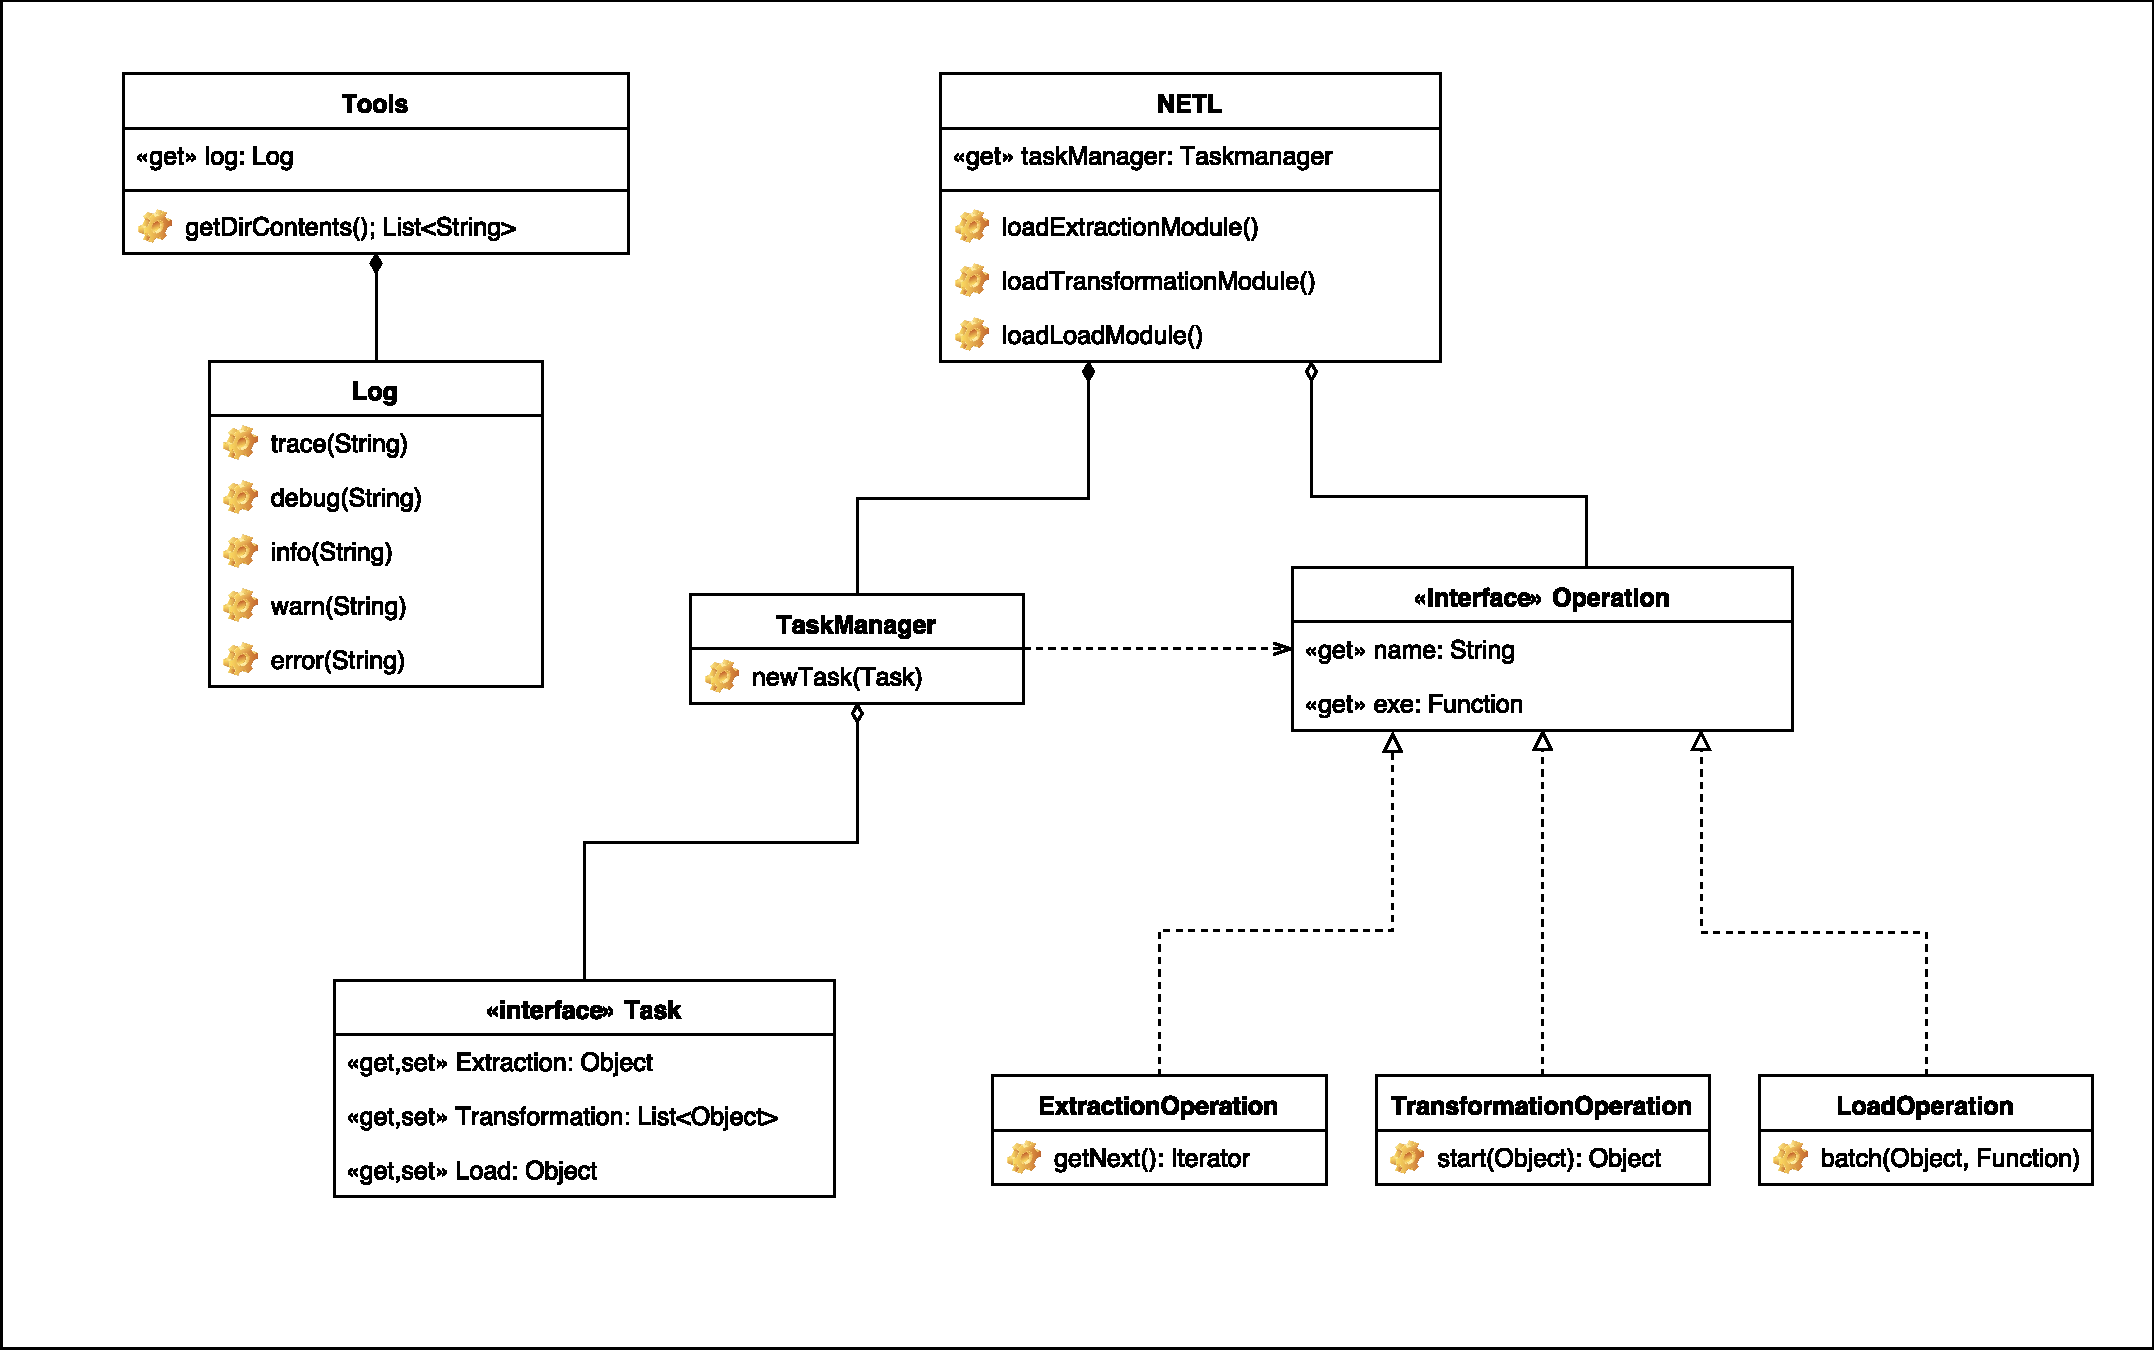
\includegraphics[scale=0.4]{./resources/figures/netlUML}
    \caption[nETL]{nETL}
    \label{nETL}
\end{figure}

Figure \ref{nETL} shows a potential architecture for a configurable component-based ETL tool. The intention of the framework is that it works on the basis of a pipeline of tasks. The framework itself is quite lightweight and comprises just the NETL, TaskManager and general purpose 'Tools' classes. For the purposes of this thesis, the framework as described by Figure \ref{nETL} has been prototyped in node.js. \textit{JavaScript} is a suitable language to prototype this application for a number of reasons:

\begin{enumerate}
    \item It has a very succinct API making it fast to write code in (i.e. it is a highly abstracted language similarly to Ruby or Python)
    \item But unlike Ruby or Python (and other high level languages), it is opinionated in that it handles IO asynchronously by default
    \item The \textit{JavaScript} implementation of object-orientation is appealing (to some developers at least)
    \item And working and learning \textit{JavaScript} is very much in line with the spirit of CouchDB and the web in general
\end{enumerate}

nETL is primarily a task-managing application, and as such, the TaskManager class is effectively the core of the application and has been implemented via the following:

\begin{minted}{javascript}
function TaskManager(extractions, transformations, loads) {
    this.tasks = {};
    this.extractions = extractions;
    this.transformations = transformations;
    this.loads = loads;
};
TaskManager.prototype.newTask = function(task) { /* ... */ };
\end{minted}

The application itself is intended to be singleton instance of \mintinline{javascript}{class NETL{}}, which provides an interface to \textit{TaskManager}, and modular extraction/transformation and load operations. Singleton's are typically implemented via the modular pattern in JavaScript, which is typically how libraries are delivered to users by package managers and invoked by \mintinline{javascript}{var library = require('library-name')();}:

\begin{minted}{javascript}
module.exports = function() {
    const _extractions = {};
    const _transformations = {};
    const _loads = {};        
    const _taskManager = new TaskManager(_extractions, _transformations, _loads);
    function _loadExtractionModule(extractionOperation){};
    function _loadTransformationModule(transformOperation){};
    function _loadLoadModule(loadOperation){};
    return {
        taskManager: _taskManager,
        loadExtractionModule: _loadExtractionModule,
        loadTransformationModule: _loadTransformationModule,
        loadLoadModule: _loadLoadModule
    };
};
\end{minted}

To achieve batches loading, \textit{JavaScript} generators are are used. As described by \cite{mozillaGenerators}, \textit{JavaScript} generators allow for quickly implementing arbitrary iterators, including iterators over generated iterators. Using open source code provided by \cite{bower16}, nETL makes use of a generator function iterate of the lines of a file, and then a higher level generator to iterate over results of the line generator to produce \textit{batches} of data that are worked through the ETL pipeline.

\begin{minted}{javascript}
/**
 * Generates lines from a flatfile
 * @yield {string} returns a single line from a flatfile
 */
function* _readLines() {
    while (pointer < filesize) {
        yield lineBuffer;
    };
};

/**
 * Generates batches of lines
 * @yield {Object[]} An array of lines
 */
function* getBatch () {
    let data = [];
    for (0..batchSize) {
        data.push(lineExtraction.getNext());
    };
    yield data;
};

// Generate lines
var lineReader = _readLines();

// Generate batches of lines
var batch = getBatch.next();
\end{minted}

Transformations are then applied to batches of lines, with the result passed to a loading function. The loading function is implemented asynchronously due to the time-cost involved when using IO (and specifically using network IO as possible with CouchDB). As batches are successfully loaded, a new batch is extracted for processing via recursion.

\begin{minted}{javascript}
(function doEtlTask(self) {
    var payload = [];

    // Extract
    batch = batchExtraction.next();
    if (batch.done) return;

    // Apply transformations
    transformations.forEach(function(t) {
        batch = t.transform(batch);
    });
    payload = batch;

    // Load
    load.batch(payload)
        .then(function(msg) {
            doEtlTask(self);
        });
})();
\end{minted}
\section{Configuration}

\textit{nETL} is configured first by the Extraction, Transformation and Load modules that a user loads, and then by the JSON configuration passed to the \textit{nETL} process during runtime to start the ETL task. The JSON configuration format is largely dependent on the E/T/L modules loaded, and in effect, has a user-defined API. Adding modules to the framework makes them available to tasks as specified by configuration objects. In this project the following modules were written and loaded, with example configurations shown in the methodology section.

\begin{enumerate}
    \item \textit{netl-extract-flatfile}
    \item \textit{netl-trans-create-obj-field}
    \item \textit{netl-trans-filter}
    \item \textit{netl-trans-text-line-to-obj}
    \item \textit{netl-trans-whitelist}
    \item \textit{netl-load-couchdb}
\end{enumerate}

As shown in \ref{nETL}, these modules must adhere to a contracts stipulated by \textit{nETL}'s module-loading interface. See \ref{appendix:netl-loading} for an example of a script that loads a module into the initiated \textit{nETL} application.

\section{Evaluation \& Results}
\subsection{Data}
Three different datasets were acquired for this project. Jane Hendry, UCT's CIO, provided data on first-time undergraduates including demographic information, matric results, and admission-acceptance test results (the \textit{FU} dataset). Stephen Marquard, the Learning Technologies Coordinator from the Center for Innovation in Learning and Teaching at UCT (the CILT) provided Sakai \textit{grade} and \textit{event} data. Each of these datasets include a student ID field, which was anonymized by Associate Professor Sonia Berman and Stephen (in the case of the \textit{event} data). The three datasets are relatable due to the anonymized student ID field which is common to all three entities.

\textit{Event} data was received for the 2016 academic year and comprises approximately 43 million rows of Sakai events of different 'event types'. This project considered only \textit{events} of type \textit{presence}, identified via an \textit{event_id} of the value \textit{281}. This translates to roughly 13 million applicable events (i.e. rows). \textit{Course grade} data was received for 2014, 2015, and 2016. The field \textit{course_id} was found to not correspond with the \textit{event} data field: \textit{site_key}, meaning that the \textit{event} and \textit{grade} data is only relatable by year and student ID, and not per individual course. Demographic data was used from 2014, 2015, 2016. Each of the years included different data fields (since 2014 registrants also had 2015 and 2016 results appended). As a result demographic data was pre-processed using Excel to normalize the entities. The grade data was also pre-processed in Excel to provide a single sheet of all three years (easier to load into a database like this); but the column names in this case remained constant. For a description of the three data entities provided by UCT refer to the appendix (\ref{appendix:data}), where a description of each field is shown and the basic filtering that was done on the CSV exports. Also in appendix \ref{appendix:data} is an example of each entity represented as JSON and as used by CouchDB. Filtering as mentioned on tables (\ref{event-data-csv}, \ref{grade-data-csv}, \ref{demographic-data-csv}) was performed in the \textit{nETL} application, specified as a \textit{transformation}. The module is shown in the appendix at \ref{netl-trans-filter}. In addition to filtering, an attribute was added to each row imported from the CSVs: \textit{\_type} - so that each document can be identified as a conceptual member of a particular entity. This additional attribute was appended to each row also via the \textit{nETL} application; an attribute \mintinline{json}{{"type\_": "<entity name>"}} was added to every CSV line extracted. Code to show how such a \textit{transformation} is achieved is included in \ref{netl-trans-create-obj-field}.
\subsection{Setting up CouchDB}
CouchDB 2.0 onwards implements clustering functionality that makes large-scale, sharded databases feasible. For the purposes of this project, clustering was tested on 3 Hetzner servers CX20 servers with indexing tested first locally on a Windows machine and then on cheap CX20 servers. The commands to provision Ubuntu Xenial and CouchDB 2.1 have been produced below. For the purposes of this project, these commands are executed via a Ruby script so as to automate the server provisioning process for any number of (existing) virtual servers. Hetzner, Digital Ocean, Google, AWS and many other cloud providers make an API available that allows for automated provisioning of \textit{n}-virtual servers, where \textit{n} is limited only by one's ability to pay!

Since virtual servers are relatively inexpensive in comparison to dedicated servers, and easier to setup, dispersed data indexing is extremely-achievable using CouchDB. CouchDB MapReduce queries could easily be dispersed among thousands of computer nodes, as could massive amounts of data. In terms of database size limits, it would theoretically be as easy working with several PB of data and 10 000 + CouchBD nodes as it is working with a small cluster.The Ruby script is called 'rCluster', with code available at \url{https://github.com/zachsa/rcluster}.

Since CouchDB 2.0 onwards is designed primarily with clustering in mind, by default databases are created with several (8) shards. A database with multiple shards per a single node is considered to be \textit{oversharded}, which is in itself fine. For the purposes of this project the default of 8 shards (\textit{q=8} in Couch-speak) is used across all servers (since the maximum number of nodes tested on is 6).

A summary of the setup script is showin in \ref{appendix:couch-setup}; this script was used to create a linux cluster for testing. Most of the work was done on a Windows machine, however, where such an elaborate install procedure is not required; there is binary available specifically for Windows.
\subsection{Loading the data}
Because CouchDB doesn't support the idea of cascade joins (as described by \cite{chandar2010}), data scrubbing such as filtering and grade-symbol-to-percent translations need to be implemented either before data is sent to CouchDB, or in the index building phase. In interest of speeding up the index-building (by far the most time consuming process in this project) filtering is implemented in the \textit{nETL} software, while logical data processing is handled in the index-building (where documents can be transformed easily via \textit{JavaScript} as directed in the index-building functions).

The extraction, transformation and loading of event and grade entities become practically identical in this case, and a single line from either CSV follows a standard transformation process of:

\[Extract line
    => JSON object
    => Filter out objects
    => Add type\_ attribute
    => whitelist wanted fields
    => load to CouchDB\]

Using \textit{nETL}, the above ETL pipeline is achieved via the following configuration format:

\begin{minted}{json}
[{
    "ID": "<name of configuration>",
    "Extraction": {
        "Name": "FLATFILE",
        "path": "path/to/file.csv",
        "skipHeaderRows": 1,
        "bufferSize": 65536,
        "batchSize": 30000,
        "startFrom": 0,
        "afterTaskRunCBs": []
    },
    "Transformations": [{
            "Name": "TEXT_LINE_TO_OBJ",
            "attributeNames": "list,of,header,values",
            "delimiter": ",",
            "textQualifier": "\"",
            "escapeChar": "\\",
            "afterTaskRunCBs": []
        },
        {
            "Name": "FILTER",
            "filterOn": {
                "field1": ["<allowed val 1>", "<allowed val 2>", "<etc>"],
                "field2": ["<allowed val 1>", "<allowed val 2>", "<etc>"]
            },
            "afterTaskRunCBs": []
        },
        {
            "Name": "CREATE_OBJ_FIELD",
            "newAttributes": [
                ["type_", "<entity type>"]
            ],
            "afterTaskRunCBs": []
        },
        {
            "Name": "WHITELIST",
            "allowedAttributes": ["list", "of", "header", "values", "type_"],
            "afterTaskRunCBs": []
        }
    ],
    "Load": {
        "Name": "COUCHDB",
        "username": "<admin>",
        "password": "<password>",
        "server": "localhost",
        "port": 5984,
        "ssl": false,
        "database": "<db name>",
        "afterTaskRunCBs": []
    }
}]
\end{minted}

TODO: Look at time complexity of the nETL modules used

\subsection{MapReduce indexes}
The idea of MapReduce allows for a varied and wide approach to data-querying in general. Application is limited somewhat in CouchDB due to it's implementation as a means of calculating a B+tree. As such it's easy to shoot yourself in the foot when building CouchDB MapReduce indexes without understanding the nature of how those indexes are stored or calculated. Also, due to the limitation of poor custom reduce function performance as mentioned previously, it is best to use built-in reduce functions, meaning that joining documents in couchDB effectively boils down to indexing different entities to a common output format via a \textit{map} function. Considering that a single \textit{map} function is used to process all documents in a database, this function should handle different cases for different entities. As mentioned previously, entity classification within the \textit{map} function is possible via the type\_ attribute that is appended to every object within the transformations performed by the \textit{nETL} app.

At the time of index calculation it is possible to group objects by common keys, but it is not possible to process those grouped keys unless you use a reduce function, in which case only simple metrics are supported. An initial attempt to produce a \textit{map} index of the form:

\begin{minted}{json}
[
    {"key": 1, "value": {"semster": 1, "grade": 67} },
    {"key": 1, "value": {"semster": 1} },
    {"key": 1, "value": {"semster": 2, "grade": 56} },
    {"key": 1, "value": {"semster": 2, "grade": 98} },
    {"key": 1, "value": {"semster": 1} },
    {"key": 1, "value": {"semster": 2} },
]
\end{minted}

And reduce grouped result (allowing for \mintinline{javascript}{rereduce=true}) via the following function:

\begin{minted}{javascript}
function(keys, values, rereduce) {
    // Return object
    var r = {
        eCountS1: 0,
        eCountS2: 0,
        gCountS1: 0,
        gCountS2: 0,
        gNormAvgS1: 0,
        gNormAvgS2: 0
    };
    if (rereduce) {
        values.forEach(function(item) {
            r.eCountS1 += item.eCountS1;
            r.eCountS2 += item.eCountS2;
            r.gCountS1 += item.gCountS1;
            r.gCountS2 += item.gCountS2;
            r.gNormAvgS1 += (item.gCountS1 * item.gNormAvgS1);
            r.gNormAvgS2 += (item.gCountS2 * item.gNormAvgS2);
        });
    } else {
        values.forEach(function(item) {
            // No item.grade means it's an event
            if (!item.grade) {
                if (item.semester === 1) {
                    r.eCountS1++
                } else {
                    r.eCountS2++
                };
                return;
            };
            // If it's a grade
            if (item.semester === 1) {
                r.gCountS1++;
                r.gNormAvgS1 += (r.gCountS1 === 1) ? item.grade : (item.gNormAvgS1 * item.grade);
            } else {
                r.gCountS2++;
                r.gNormAvgS2 += (r.gCountS2 === 1) ? item.grade : (item.gNormAvgS2 * item.grade);
            };
        });
    };
    return r;
};
\end{minted}

After almost 10 hours of waiting for the index to build, the calculation was canceled. it's hard to know what the bottlenecks of calculating the index using this method are; Jan Lehnardt mentioned (see \ref{appendix:slack3}) that the majority of the work done in the indexing process is by the \textit{map} process. However, it should be noted that per an student ID there could be as many as 8 000 objects in the \textit{value} array, so that could also be a factor. In terms of time complexity, this query superficially seems fine - approximately  $ O(n^2) $ TODO.

On "re-imagining" the MapReduce query to make use of CouchDB's built-in \_sum function to aggregate several metrics, the map function needs to output \textit{key:value} pairs of a slightly different form:

\begin{minted}{json}
[
    { "key": 1, "value": ["<iEvCountS1>", "<iEvCountS2>", "<iGrCountS1>", "iGrCountS2", "<fGrTotS1>", "<fGrTotS2>"] },
    { "key": 1, "value": [0, 1, 0, 0, 0, 0] },
    { "key": 1, "value": [0, 1, 0, 0, 0, 0] },
    { "key": 1, "value": [1, 0, 0, 0, 0, 0] },
    { "key": 1, "value": [0, 0, 0, 1, 0, 45] },
    { "key": 1, "value": [0, 0, 1, 0, 76, 0] },
    { "key": 2, "value": [0, 0, 1, 0, 50, 0] },
]
\end{minted}

CouchDB's built-in \_sum \textit{reduce} aggregates the above result to:

\begin{minted}{json}
[
    { "key": 1, "value": [1, 2, 1, 1, 76, 45] },
    { "key": 2, "value": [0, 0, 1, 0, 50, 0] },
]
\end{minted}

which is a suitable join for grade analysis. The full \textit{Map} and \textit{Reduce} functions to achieve this are described below and is approximately $ O(n) $... TODO. Some filtering is done in the \textit{Map} function that could just as easily have been applied to the data within the \textit{nETL} process. Logic on handling non-numerical percents as described previously is handled within the map function.

\begin{minted}{javascript}
// Map function
/**
 * outputs: key:[eCountS1, eCountS2, gCountS1, gCountS2, gSumAvgS1, gSumAvgS2]
 * @param {Object} doc CouchDB document passed to Map function
 */
function(doc) {
    var output = [0, 0, 0, 0, 0, 0];
    var disallowedPercents = ['ATT', 'DE', 'GIP', 'LOA', 'OS', 'OSS', 'PA', 'SAT', 'UNS', ''];
    var allowedSuffixes = ["S", "F", "W", "H", "L", "P"];
    switch (doc.type_) {
        case 'courseGrade':
            var semester = (doc.CourseSuffix || 'N').toUpperCase();
            if (allowedSuffixes.indexOf(semester) >= 0) {
                var p = doc.Percent || '';
                // If p not a number, try convert
                if (typeof p !== 'number') {
                    if (typeof p !== 'string') return;
                    var newP = p.toUpperCase().trim();
                    if (disallowedPercents.indexOf(p) >= 0) return;
                    switch (newP) {
                        case 'AB':
                            p = 40;
                            break;
                        case 'F':
                            p = 40;
                            break;
                        case 'DPR':
                            p = 20;
                            break;
                        case 'INC':
                            p = 20;
                            break;
                        case 'UF':
                            p = 30;
                            break;
                        case 'UP':
                            p = 50;
                            break;
                        default:
                            p = parseFloat(p.substring(0, p.length - 1));
                            if (isNaN(p)) return;
                            break;
                    };
                };
                if (semester === 'F' || semester === 'L') {
                    output[2] = 1;
                    output[4] = p;
                } else if (semester === 'S' || semester === 'P') {
                    output[3] = 1;
                    output[5] = p;
                } else {
                    output[2] = 1;
                    output[3] = 1;
                    output[4] = p;
                    output[5] = p;
                };
                emit(doc.anonIDnew, output);
            };
            break;
        case 'vulaEvent':
            var date = (new Date(doc.event_date)).getTime();
            var midDate = 1468792800000 // Sunday, July 17, 2016 10:00:00 PM
            var semester = (date - midDate >= 0) ? 2 : 1;
            if (semester === 1) {
                output[0] = 1;
            } else {
                output[1] = 1;
            };
            emit(doc.uct_id, output);
            break;
        default:
            break;
    };
};

// Reduce function
_sum // Built-in function
\end{minted}

\subsection{Index retrieval}
Due to the nature of B+tree indexes in CouchDB retrieving view data is very quick - this is the benefit of CouchDB's MapReduce implementation over non-indexed output such as Hadoop. The view data is formatted as a JSON array of \textit{[key,value]} pairs. To use the view data outside of viewing it in a browser, a translation step is required since CouchDB doesn't offer tool to export or save output. For the purposes of this project output is required in the \textit{CSV} format so as to facilitate further data analysis using stats programs, Excel, saving the output in a data warehouse, etc.

Converting CouchDB index output to \textit{CSV} is possible in this project using the \textit{nETL} application. Such a \textit{task} involves an extraction from CouchDB's \textit{:db/\_view/viewName?reduce=true\&group=true} HTTP endpoint, a translation from JSON documents to CSV rows and a \textit{loading} process to a flatfile destination. Such a configuration might look as indicated below. To achieve this a \textit{COUCH\_INDEX} module needs to be written and loaded into \textit{nETL}. The \textit{FlATFILE} module already exists for purposes other than this project, although it's not discussed within the project itself.

\begin{minted}{json}
[{
    "ID": "<name of configuration>",
    "Extraction": {
        "Name": "COUCH_INDEX",
        "uri": "localhost:5984/msc/_design/db/_view/student-grades?group=true&reduce=true",
        "afterTaskRunCBs": []
    },
    "Transformations": [{
            "Name": "OBJ_TO_CSV",
            "delimiter": ",",
            "textQualifier": "\"",
            "escapeChar": "\\",
            "afterTaskRunCBs": []
        }
    ],
    "Load": {
        "destinationType": "FLATFILE",
        "skipBlankLines": true,
        "path": "path/to/download/results.csv",
        "afterTaskRunCBs": []
    }
}]
\end{minted}

As of CouchDB 2.1 there is the concept of a \textit{list} functions, although as noted previously and confirmed by personal communication with Jan Lehnardt the current CouchDB PMC chair (see \ref{appendix:slack4}), while this feature is not going to be removed it may fall by the wayside without additional support. But with support in the current implementation of CouchDB they represent a more time-effective of retrieving information from CouchDB indexes than using the \textit{nETL} app - and this is the solution that this project show cases. \textit{List} functions, like \textit{MapReduce} indexes, are defined in design documents. The functions iterate the rows of an index to a user in the specified format along with any transformations. Since index results are guaranteed to be ordered by key, this is powerful and allows for combining result steps of documents for adjacent keys if required. In this project a list function is simply used to enable users to download the values produced by the \textit{student-grades} view in CSV format, and is defined be the code below. This function is called via the URI \textit{host:5984/db/\_design/name/\_list/listname/viewname?group=true\&reduce=true}. All of the parameters available to the index retrieval endpoint (\textit{\_view/...}) are available when the view is called by the list function, including specifying an array of keys if only a subset of the index results are required. Time complexity of the list function is approximately $ O(n) $ TODO.

\begin{minted}{javascript}
function(head, req) {
    provides('csv', function() {
        var headers = "Student ID (anonymized),\
        Presence Events S1,\
        Presence Events S2,\
        Grade Count S1,\
        Grade Count S2,\
        Grade Sum S1,\
        Grade Sum S2,\
        Grade Avg S1,\
        Grade Avg S2";
        send(headers);

        while (row = getRow()) {
            var id = row.key;
            var value = row.value;
            var eCountS1 = value[0];
            var eCountS2 = value[1];
            var gCountS1 = value[2];
            var gCountS2 = value[3]
            var gSumS1 = value[4];
            var gSumS2 = value[5];
            var gAvgS1 = (gCountS1 > 0) ? (gSumS1 / gCountS1) : "";
            var gAvgS2 = (gCountS2 > 0) ? (gSumS2 / gCountS2) : "";
            var line = "\n" + id + "," + eCountS1 + "," + eCountS2 + "," + gCountS1 + "," + gCountS2 + "," + gSumS1 + "," + gSumS2 + "," + gAvgS1 + "," + gAvgS2;
            send(line);
        };
    });
};
\end{minted}

\section{Discussion}
\section{Results}
An important property of any benchmarking method is the variance of the datasets from which these benchmarks are drawn. Small variance will magnify small discrepancies between students and as such does not provide a useful means of assessing students for university admission. An ideal benchmark has a high degree of correlation with a large variance. Obviously benchmarking methods should be applicable to as large a group of students as possible (for example, although additional mathematics may be a good means of assessing incoming student's abilities, it is useless since so few students take this subject in matric).

\subsection{Variance}

\subsection{Benchmark / Grade Correlation}
Correlation between the Grades and various combinations of the Benchmarks data shows that compared to Gr12 results, the NBT scores correlate better with CSC1015F performance. The highest correlation between benchmarking and CSC1015F course results occurs when the NBT scores are averaged, with either the NBT QL or NBT Mth (or both) scores double weighted; such a correlation is 0.50, which is considered a moderate correlation.

Because none of the students have grades for the ``G 12 Mth Lit'' and ``G12 Mth Adv'' columns who attended the CSC1015F course, these benchmarks are not taking into account.

\subsection{LMS Usage}
Because the event data doesn't contain a foreign key to the grade entities, it is only possible assess the count of presence events for all sites in relation to the CSC1015F site. This isn't particularly useful, and perhaps is the main reason that no correlation is found. However this analysis is useful in demonstrating how such a correlation can be performed using CouchDB making such an analysis somewhat worthwhile.


Taking the NBT QL benchmark as an example (which has a comparatively high correlation with course grades compared to other benchmarks), the \( \delta \) class rank of benchmark score vs grade score is plotted against presence event count of each student in \ref{fig-delta-rank} for a visual feel of how the correlation analysis plots. The correlation between course grades (for CSC1015F) and LMS usage is relatively insignificant according to these results.

\begin{figure}[H]
    \centering
    % \begin{mdframed}
    % \centering
    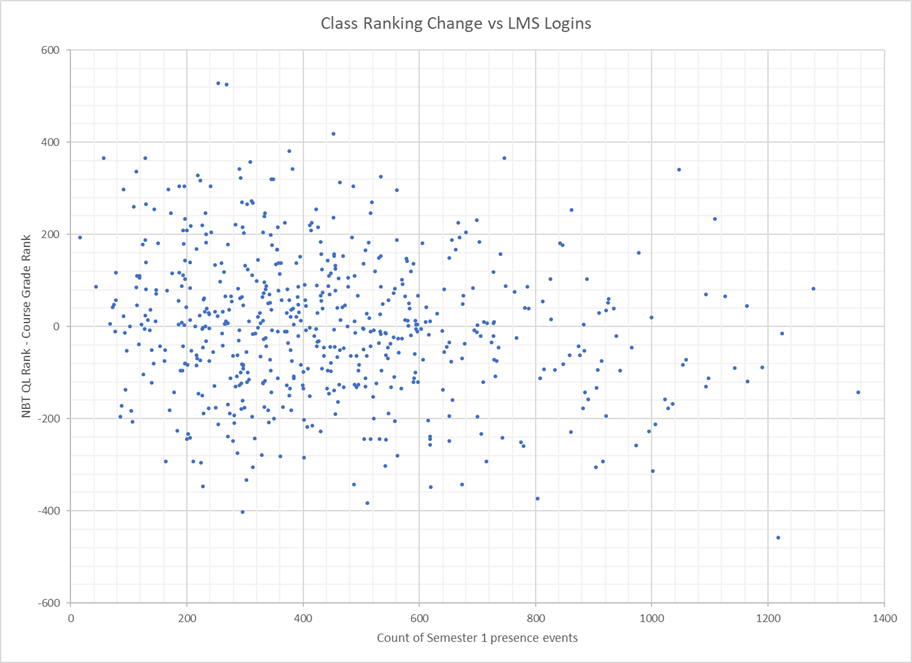
\includegraphics[scale=0.6]{./resources/figures/delta-class-rank.png}
    % \end{mdframed}
    \caption[\( \delta \) class rank vs LMS Logins]{\textbf{Figure \ref{fig-delta-rank}: \( \delta \) class rank vs LMS Logins.} An example of the correlation between \( \delta \) NBT QL ranking scores/course grades compared to LMS usage. As shown in Table \ref{tbl-correlation-variance}, the correlation coefficient between these two datasets is 0.17.}
    \label{fig-delta-rank}
\end{figure}

\section{Conclusion}
1. However CouchDB itself has an opinionated implementation of MapReduce - which is used to build B+indexes instead of result sets as in hadoop. As such CouchDB's MapReduce is only useful when querying for analytics of a numerical nature.

2. CouchDB query times go down with more cluster nodes.

3. CouchDB is good for ... xxx
\subsection{Future work}

\begin{enumerate}
    \item test on much larger cluster sizes
    \item test with different n,q values
    \item UI research for nETL - the JSON config is pretty cool. maybe non-techinical people could use it
    \item test same cluster sizes on different linux VMs (different amount of power per pc)
\end{enumerate}
\section*{Acknowledgments}
I would like to give special thanks to my project supervisor Associate Professor Sonia Berman - an extremely patient supervisor who had the foresight to push me (at great effort) in the direction that resulted in a completed MSc. I would also like to thank her for the effort she put in in terms of data acquisition and guiding me in designing the research topic. I would also like to thank Jane Hendry and Stephen Marquard for providing the data exports and scrubbing that such exports required. And lastly I would like to thank the many people who helped me with insights into the thesis topic and the technologies I used. Including: Stephanie Honchell, Patrick DeSomma, Guy Bedford, and many of the CouchDB community who took the time to reply to my messages over Slack.
\newpage

% Bibliogrpahy
\bibliographystyle{plain}
\bibliography{bibliography/msc_citations}

% Appendix
\begin{appendix}
    \section{Appendix}
    \subsection{Slack conversations}
\label{appendix:slack}

\subsubsection{October 25 2017}
zach [12:13 PM]
Hi. What would cause CouchDB rereduce=true param when running a reduce task?

rnewson (IRC) APP [12:25 PM]
couchdb stores the result of the reduce function on internal b+tree nodes of the view index. rereduce is true when we're higher up in the tree and need to know the reduction of a group of previous reductions.

[12:25]
so it happens when you have more than a handful of documents and your reduce function will only work correctly if you do the right thing for rereduce false and true cases.

[12:26]
when rereduce is true, the keys param is null and the values array is the output of previous calls to your reduce function.

zach [12:30 PM]
thank you. that means that a reduce function needs to work with an input of either the map output or it's reduce output? Is there a term for this kind of function? I feel like there should be...

rnewson (IRC) APP [12:31 PM]
yes, the contract for a reduce function is that it must work for both types of input, and the third parameter tells you which you're doing.

[12:31]
there are implementations where the logic is the same for both types, of course.

[12:32]
"return sum(values);" for example

zach [12:48 PM]
Thanks again! I'm not super familiar with the b-trees, but my understanding is that if you are higher up on such a tree, that the key you are looking for exists lower down? Would it be correct to say that rereduce is a means of appending to a reduce functions output that already exists? If the entire index was calculated from scratch then, could you assume that rereduce will always be false since grouped output of the map function means that a reduce function will NOT reprocess the same keys?

rnewson (IRC) APP [12:51 PM]
no, you cannot assume that

    [12:51]
rereduce param will be set to false and true for any database above 10 documents or so

    [12:51]
write your reduce function accordingly, that's the contract

zach [12:54 PM]
thank you

\subsubsection{October 31 2017}
zach [3:53 PM]
at the risk of sounding like a repetitive novice... what is wrong with indexes that get bigger and bigger? Is it best to avoid them because a) there is almost always a better way of doing something? or b) they have some other effect on the CouchDB process (other than whatever overhead is required to use a larger-than-requried index)

rnewson (IRC) APP [3:57 PM]
'bigger and bigger'?

jan [4:03 PM]
@zach not sure what you mean, indexes are expected to grow with more documents

zach [4:22 PM]
writing a reduce function I sometimes get a warning that reduce output is not shrinking fast enough - in this case i can either rewrite my reduce function or turn off the setting. As you mentioned previously @jan, option 1 (rewriting) is definitely the way to go. But what is the reason for this? Is it because a reduce function that doesn't shrink output requires continuous balancing of the B+ tree which means poor performance? (i don't have a background in data structures). what are the theoretical problems of in a reduce function like this: function(keys, values, rereduce){return values (with code to do the same in the rereduce)} if there was an unlimited amount of hardrive space available.

[4:23]
I know this is a 'relational' approach.. and that there are better options. but I'm still interested in why

jan [4:49 PM]
that reduce function will copy all values from the leaves of the b-tree into the root node, and all intermediate nodes get their share of leaves copied in as well. You’re effectively stacking a reverse tree on top of the actual tree, approaching $ O(n^2) $ or worse performance and disk use.

zach [4:51 PM]
ah. thank you

jan [4:55 PM]
I.e. it subverts everything an index is meant to do

rnewson (IRC) APP [5:12 PM]
I'm curious to know what the reduce function is

jan (IRC) APP [5:13 PM]
" a reduce function like this: function(keys, values, rereduce){return values (with code to do the same in the rereduce)}"

afinne [5:33 PM]
zach, just to double check: you are aware that a reduce function is not mandatory?

zach [5:42 PM]
Hi @afinne - yes. why do you ask? (I don't think I was able to group without the reduce function)

Wohali (IRC) APP [5:43 PM]
just use a built-in reduce like \_sum

[5:43]
if all you want is grouping

zach [5:43 PM]
if I say group=true and reduce = false I get an error

rnewson (IRC) APP [5:44 PM]
yes, you need a reduce if you want to group.

[5:44]
though 'return null' is sufficient

zach [5:45 PM]
would that guarantee all values returned for a particular key?

[5:48]
I re-wrote the reduce function to aggregate. though I must have done something wrong since 5 hours later it's still calculating

...

[5:49]
and the database is only about 3.5GB

rnewson (IRC) APP [5:49 PM]
well, you'll @fabsolute least get compound rounding errors from the divide

    [5:49]
but the whole thing looks wrong tbh

    [5:49]
what does the map look like? what does a doc look like?

[5:51]
hm, I bet you could get the built-in's to do this for you

    [5:51]
if you emitted an array as your value in map, then \_sum will sum each item, etc

    [5:52]
for an average, you should calculate both values and then divide @fabsolute the client, you can't do it as you go

    [5:52]
and a note of caution, if any of your values happen not to be numbers, you'll end up doing string concatenation and blowing things up that way

    [5:53]
so I suggest typeof(number) checks

zach [5:53 PM]
thanks. the map function looks like this: (url)

...

zach [6:03 PM]
Thanks for pointing out the rounding and average points @rnewson. I think I understand how I could use the \_sum, but I don't know how I would include the average

rnewson (IRC) APP [6:04 PM]
you couldn't, but you could include the numbers you need to calculate the average from the result of the \_view request

    [6:05]
that is, don't bother calculating r.gAvgS1 or r.gAvgS2 in the view

    [6:05]
just calculate it from the other two fields from the view response

zach [6:07 PM]
oh. i guess i could just sum the grades percent and divide by total grades at the end.

rnewson (IRC) APP [6:07 PM]
aye

    [6:08]
the built-in \_stats endpoint would give you the sum and count of the values, which you could then use to get mean average

    [6:08]
afk

\subsubsection{November 1 2017}
zach [12:25 PM]
Question @rnewson - thanks for those pointers yesterday. it took just over an hour to finish indexing the MapReduce view using the \_sum reduce function. In an unrelated note, I remember reading somewhere that the default reduce functions run much more efficiently than custom reduce function? why is this? i also recall someone mentioning (I think it was on this channel) that the reduction phase is done by the main erlang process. Does this mean that reduction is not done in parallel? i.e. the map functions are computed using instances of couchjs, but the reduce function is done via a single process?

zach [12:48 PM]
ah. i see why there is a performance difference here: http://docs.couchdb.org/en/2.1.0/maintenance/performance.html\#builtin-reduce-functions. I'd still be interested to know if the reduce function is done by many 'reducers'

jan [12:55 PM]
per view build, it is sequential, optimising for write IO / on a sharded system, view builds are per-shard

zach [1:10 PM]
is it correct to say that for a particular view: per shard, map indexes are calculated in parallel (multiple couchjs processes), followed by a single instance of the reduce function (a single process)? i.e. a database running as a single node with 8 shards would have at most 8 reduce functions running? So theoretically speaking increasing shards would decrease the time taking to build MapReduce indexes?

[1:11]
I now understand what I see 8 instances of the couchjs process in Windows task manager

jan [1:11 PM]
the reduce, especially built-in reduce is not likely to be factor in view build times.

[1:11]
oh

    [1:11]
windows

    [1:11]
windows has extra slowness added to it

zach [1:12 PM]
why is that?

jan [1:13 PM]
Windows isn’t very good at unix-style inter process communication

zach [1:14 PM]
so there is an overhead every time a map process is spawned and returned...

jan [1:15 PM]
it’s less the spwning, and more the i/o

\subsubsection{November 2 2017}
zach [10:57 AM]
will list functions be included in future versions of CouchDB? I saw a thread that they are considered as part of CouchApps and may not. I kinda love them

jan [11:02 AM]
@zach we have no plans to remove them, but they may fall by the wayside. Nobody has worked on that in 5+ years, and it’s not something we recommend anyone using

\subsubsection{November 7 2017}
zach [11:46 AM]
when I look at data/shards/... I see that my database is split amongst 8 shards on my single node setup. How does Couch distribute documents to each shard (i'm using the default \_id generator). When in clustered mode, can I assume that data gets distributed amongst shards evently?

Wohali (IRC) APP [11:48 AM]
it's based on a hash of the document

[11:49]
which should be random enough to ensure equal distribution

zach [11:49 AM]
Thank you

Wohali (IRC) APP [11:49 AM]
in clustered mode, in a 3 node cluster, every node gets a copy of your document

[11:49]
so all 8 shards are stored on all 3 nodes (total 24 shards)

zach [11:49 AM]
that's if n=3 though?

[11:49]
if I configure n=1, q=8

    [11:50]
this is to see if increasing number of nodes in a cluster reduces index time... should it?

[11:51]
if n \textgreater 1, would that result in an index being calculated more than once/

[11:51]
?

Wohali (IRC) APP [11:52 AM]
i'm too tired to answer that right now

    [11:52]
maybe someone else can help you

    [11:52]
i have been up for 24 hours.

zach [11:54 AM]
i imagine that increasing nodes would result in decreasing index creation time since map output is calculated per node. and I would imagine that data copies don't get their own indexes. thanks :slightly\_smiling\_face:. have a good sleep

Wohali (IRC) APP [11:57 AM]
map output is calculated per shard, per copy

    [11:57]
on every node

    [11:57]
8 shards on a node = 8 couchjs processes

zach [11:58 AM]
so if n=3, then three copies of each view are calculated?

[11:59]
is that to increase availability of index retrievals?

[12:01]
I think Jan mentioned that it was a single couchjs process per reduce function, but many couchjs processes per map function. i saw this on my windows pc - n = 1 with 8 shards, there are at first many more than 8 couchjs processes running, and then only 8 processes running

Antonio [1:26 PM]
joined \#general.

rnewson (IRC) APP [3:50 PM]
'but many couchjs processes per map function' - nope.

[3:50]
each view shard is built separately exactly as a view used to build in couchdb \textless 2.0.

[3:50]
that is, sequentially in \_changes order until current.

zach [3:57 PM]
oh. sorry i misunderstood.

[3:57]
thank you

\subsubsection{November 20 2017}
zach [1:52 PM]
Hi - is there anyway to simulate a SQL 'Window' function in CouchDB? i.e. could I do something like `rank() over(partition by someClassification order by someNumber desc)`. Since I can't guarantee that in my reduce function I will have all the values for a particular key, I'm assuming 'no'?

[1:53]
I can do this in the list function, i know that

jan [2:45 PM]
or outside of CouchDB with the reduce result. Would avoid list funs

\subsubsection{November 24 2017}
zach [11:40 AM]
Hi. In a Map query, I created a variable `key` that I would then adjust and emit several times: `function(doc) {var key = [it1, it2, it3]; var arr = ["a", "b", "c", etc]; arr.forEach(function(val) {key[1] = val; emit(key, ...)})}`. but i found that the `forEach` loop didn't work as expected. It seemed that the variable `key` was in a global scope that was shared by separate instances of the map function -i.e. all the keys emitted were the last string in `arr`. Is this supposed to be the case? (edited)

jan [11:45 AM]
@zach can you share the full map fun code in a pastie service somewhere? (don’t paste here pls)

rnewson (IRC) APP [11:49 AM]
ah, I can believe that

    [11:49]
emit(key,value) simply builds an array that we return @fabsolute the end

    [11:49]
so if you're modifying a variable that you emitted, it won't work as you expect

    [11:50]
though of course in your case you're also making 'key' have a scope outside of the forEach anyway

zach [11:52 AM]
the full map function is available here: https://gist.githubusercontent.com/zachsa/52fa64fd0cc85de7b0f7fb7601aaba53/raw/ec800a79e12920f22d2d6da5d87ee020ccd44379/map%2520function

[11:53]
thank @rnewson - at the end of the map function?

rnewson (IRC) APP [11:53 AM]
after the end of the map function

    [11:54]
there's an array declared before we call your map function, any calls to emit() add items to it.

[11:54]
\_if\_ your function returns successfully, that array is then marshalled back to couchdb erlang side

    [11:54]
this is why an error in your map function causes none of your emits to appear in the view.

[11:54]
but also why you're seeing this effect

zach [11:58 AM]
oh ok. so per an execution of a map function, if i emit the variable 'key' several times it's just a reference to a single object - and the same for value in the case of the function (though I don't change the value variable after I emit). Thanks!

rnewson (IRC) APP [11:58 AM]
https://github.com/apache/couchdb/blob/master/share/server/views.js
    \subsection{CouchDB design documents}
\label{appendix:designDoc}

\subsubsection{\textit{Map} and \textit{Reduce} function contracts}
\begin{minted}{javascript}
/**
 * Map function
 * @param  {Object} doc Each document in the database is passed in turn to the function
 * @return {null} Nothing is returned - key:value pairs are emitted (multiple pairs can be emitted per document)
 */
function(doc) {
    emit(someKey, someValue);
};

/**
 * Reduce function
 * @param  {Object[]} [keys] A list of [key, docId] pairs - key as from the map function, and key from the original doc
 * @param  {Object[]} values Output from the map function, or from the reduce function
 * @param  {Boolean} [rereduce] Indicates whether values are output from the map (rereduce = false) or reduce (rereduce = true) function
 * @return {[type]}
 */
function(keys, values, rereduce) {
    if (rereduce) {
        return // ...someValue
    } else {
        return // ...someValue    
    };
};
\end{minted}

\subsubsection{A sample design document}
\begin{minted}{json}
{
    "_id": "_design/sample",
    "_rev": "xxxxx",
    "language": "javascript",
    "views": {
        "view1": {
            "map": "function(doc) { ... }",
            "reduce": "function(keys, values, rereduce) { ... }"
        },
        "view2": {
            "map": "function(doc) { ... }",
            "reduce": "_stats"            
        }
    },
    "shows": {
        "show1": "function(doc, req) { ... }",
        "show2": "function(doc, req) { ... }"
    },
    "lists": {
        "listFunc1": "function(head, req) { ... };",
        "listFunc2": "function(head, req) { ... };"
    },
    "updates": {
        "update1": "function(doc, req) { ... }",
        "update2": "function(doc, req) { ... }"
    },
    "filters": {
        "filter1": "function(doc, req) { ... }",
        "filter2": "function(doc, req) { ... }"
    },
    "validate_doc_update": "function(newDoc, oldDoc, userCtx, secObj) { ... }"
}

\end{minted}
    \subsection{\textit{nETL}}
\label{appendix:netl}

\subsubsection{Main class}
\label{appendix:netl-main}
\begin{minted}{javascript}
module.exports = function() {
    const _extractions = {};
    const _transformations = {};
    const _loads = {};        
    const _taskManager = new TaskManager(_extractions, _transformations, _loads);
    function _loadExtractionModule(extractionOperation){};
    function _loadTransformationModule(transformOperation){};
    function _loadLoadModule(loadOperation){};
    return {
        taskManager: _taskManager,
        loadExtractionModule: _loadExtractionModule,
        loadTransformationModule: _loadTransformationModule,
        loadLoadModule: _loadLoadModule
    };
};
\end{minted}

\subsubsection{TaskManager}
\label{appendix:netl-taskmanager}
\begin{minted}{javascript}
function TaskManager(extractions, transformations, loads) {
    this.tasks = {};
    this.extractions = extractions;
    this.transformations = transformations;
    this.loads = loads;
};
TaskManager.prototype.newTask = function(task) { /* ... */ };
\end{minted}

\subsubsection{Extraction}
\label{appendix:netl-extraction}
\begin{minted}{javascript}
/**
 * Generates lines from a flatfile
 * @yield {string} returns a single line from a flatfile
 */
function* _readLines() {
    while (pointer < filesize) {
        yield lineBuffer;
    };
};

/**
 * Generates batches of lines
 * @yield {Object[]} An array of lines
 */
function* getBatch () {
    let data = [];
    for (0..batchSize) {
        data.push(lineExtraction.getNext());
    };
    yield data;
};

// Generate lines
var lineReader = _readLines();

// Generate batches of lines
var batch = getBatch.next();
\end{minted}

\subsubsection{The engine}
\label{appendix:netl-engine}
\begin{minted}{javascript}
(function doEtlTask(self) {
    var payload = [];

    // Extract
    batch = batchExtraction.next();
    if (batch.done) return;

    // Apply transformations
    transformations.forEach(function(t) {
        batch = t.transform(batch);
    });
    payload = batch;

    // Load
    load.batch(payload)
        .then(function(msg) {
            doEtlTask(self);
        });
})();
\end{minted}

\subsubsection{}
\label{appendix:netl-loading}
\begin{minted}{javascript}
// Load the module into memory
memoryObject[userModule.name] = userModule.exe;
// Invoke the module's closure
var loadedModule = memoryObject[userModule.Name].call(userModule);
// Genrate batch from extraction module
var batch = loadedModule.getNext()
// Do transformations on batch
batch = loadedModule.transform(batch);
// Load transformed batch
load.batch(batch).then(function(msg) {}).catch(function(msg) {});
// An example userModule (an extraction module)
userModule = (function() {
    function exe(configurationObj) {
        function getNext() { /* ... */};
        return {
            getNext: getNext
        };
    };
    return {
        name: "MODULE_NAME",
        exe: exe
    };
})();
\end{minted}
    \subsection{CouchDB}

\subsubsection{Setup script}
\label{appendix:couch-setup}
\begin{minted}{sh}
# Set hostname of server
hostname <hostname>; rm /etc/hostname; touch /etc/hostname; echo <hostname> >> /etc/hostname; chmod 466 /etc/hostname;

## Install basic tooling 
# GCC collection (GNU make and GNU compiler tools)
apt-get update
apt-get install build-essential -y

# Update openssl to 1.0.2l
cd /usr/src
wget https://www.openssl.org/source/openssl-1.0.2l.tar.gz
tar -zxf openssl-1.0.2l.tar.gz
cd openssl-1.0.2l
./config
make
make test
make install
mv /usr/bin/openssl /root/
ln -s /usr/local/ssl/bin/openssl /usr/bin/openssl

# Python
apt-get update
apt-get install python -y

# libcurl
apt-get update
apt-get install libcurl4-openssl-dev -y

# ICU
apt-get update
apt-get install libicu-dev -y

# Pre-seed debconf to answer CouchDB installation wizard automatically
debconf-set-selections <<< 'couchdb couchdb/bindaddress string 0.0.0.0'
debconf-set-selections <<< 'couchdb couchdb/cookie string monster'
debconf-set-selections <<< 'couchdb couchdb/mode string clustered'
debconf-set-selections <<< 'couchdb couchdb/nodename string couchdb@<hostname>'
debconf-set-selections <<< 'couchdb couchdb/adminpass password <password>'
debconf-set-selections <<< 'couchdb couchdb/adminpass_again password <password>'

# register CouchDB package with the server package manager and install
echo 'deb https://apache.bintray.com/couchdb-deb xenial main' | sudo tee -a /etc/apt/sources.list
curl -L https://couchdb.apache.org/repo/bintray-pubkey.asc | sudo apt-key add -
apt-get update
apt-get install couchdb -y

# And then once those commands have been run to setup all the CouchDB nodes, the CouchDB cluster can be configured using a few commands on any one node (temporarily referred to as the CoOrdinatingNodeHost)
# Run these two lines to add a node to the CouchDB cluster
curl -X POST -H \"Content-Type: application/json\" http://<username>:<password>@<CoOrdinatingNodeHost>:<port>/_cluster_setup -d '{\"action\": \"enable_cluster\", \"bind_address\":\"CoOrdinatingNodeHost\", \"username\": \"<username>\", \"password\":\"<password>\", \"port\": <port>, \"node_count\": \"<intented node count>\", \"remote_node\": \"<remote hostname>\", \"remote_current_user\": \"<username>\", \"remote_current_password\": \"<password>\" }'
curl -X POST -H \"Content-Type: application/json\" http://<username>:<password>@<CoOrdinatingNodeHost>:<port>/_cluster_setup -d '{\"action\": \"add_node\", \"host\":\"<remote hostname>\", \"port\": \"<port>\", \"username\": \"<username>\", \"password\":\"<password>\"}'

# Finalize the cluster setup
curl -X POST -H \"Content-Type: application/json\" http://<username>:<password>@<CoOrdinatingNodeHost>:<port>/_cluster_setup -d '{\"action\": \"finish_cluster\"}'
\end{minted}
    \subsection{Data}
\label{appendix:data}
\subsubsection{Sakai Events}
\label{appendix:sakai-events}
\begin{table}[]
    \centering
    \caption{Sakai event data}
    \label{event-data-csv}
    \begin{tabular}{llll}
        Field name     & Field type & Notes                   & Include in scrape \\ \hline
        event\_date    & date       &                         & \cmark            \\
        event\_id      & int        & Filtered: only 281 used & \cmark            \\
        uct\_id (anon) & int        &                         & \cmark            \\
        site\_key      & int        &                         & \cmark            \\
        ref            & string     &                         & \xmark            \\ \hline
    \end{tabular}
\end{table}

An example of an event row as a JSON document
\begin{minted}{json}
{
  "_id": "000e569ee321b915bae59fe62e0051e3",
  "_rev": "1-7112afce121087818c33ebfd0fd7fed7",
  "event_date": "2016-04-17T14:04:20.000Z",
  "event_id": 281,
  "uct_id": 3018438,
  "site_key": 2297,
  "type_": "vulaEvent"
}
\end{minted}

\subsubsection{Grade data}
\label{appendix:grade-data}
\begin{table}[]
    \centering
    \caption{Grade data}
    \label{grade-data-csv}
    \begin{tabular}{lll}
        Field name       & Field type & Include in scrape \\
        DownloadedDate   & date       & \xmark            \\
        RegAcadYear      & int        & \cmark            \\
        RegTerm          & int        & \xmark            \\
        anonIDnew        & int        & \cmark            \\
        RegProgram       & string     & \xmark            \\
        RegCareer        & string     & \xmark            \\
        Degree           & string     & \xmark            \\
        DegreeDescr      & string     & \xmark            \\
        Subject          & string     & \xmark            \\
        Catalog.         & string     & \xmark            \\
        Course           & string     & \cmark            \\
        CourseSuffix     & string     & \xmark            \\
        Session          & string     & \xmark            \\
        Percent          & string     & \cmark            \\
        Symbol           & string     & \xmark            \\
        UnitsTaken       & int        & \xmark            \\
        CourseID         & int        & \xmark            \\
        CourseDescr      & string     & \xmark            \\
        CourseCareer     & string     & \xmark            \\
        Faculty          & string     & \xmark            \\
        Dept             & string     & \xmark            \\
        MaximumCrseUnits & int        & \xmark            \\
        CourseCount      & int        & \xmark            \\
        CourseLevel      & int        & \xmark            \\
        CESM             & int        & \xmark            \\
        Sub-CESM         & int        & \xmark            \\
    \end{tabular}
\end{table}

An example of a course grade as a JSON document:

\begin{minted}{json}
{
  "_id": "7530f4eed7e6bc3ef0d99a53be8ba9a2",
  "_rev": "8-232d0cf39728d41b4c5935f12469209d",
  "RegAcadYear": 2016,
  "RegTerm": 1161,
  "anonIDnew": 1,
  "RegCareer": "UGRD",
  "Degree": "QHB002",
  "Course": "PHI1010S",
  "CourseSuffix": "S",
  "Percent": "55",
  "CourseID": 109157,
  "Dept": "PHI",
  "type_": "courseGrade"
}
\end{minted}

\subsubsection{Demographic data}
\label{appendix:demographic-data}
\begin{table}[]
    \centering
    \caption{Demographic data}
    \label{demographic-data-csv}
    \begin{tabular}{llll}
        Field name             & Field type & Notes                           & Include in scrape \\ \hline
        anonIDnew              & int        &                                 & \cmark            \\
        Career                 & string     & filtered: only UGRAD used       & \xmark            \\
        Citizenship Residency  & string     & filtered: only SA citizens used & \xmark            \\
        SA School              & string     &                                 & \xmark            \\
        Eng Grd12 Fin Rslt     & string     &                                 & \cmark            \\
        Math Grd12 Fin Rslt    & string     &                                 & \cmark            \\
        Mth Lit Grd12 Fin Rslt & string     &                                 & \cmark            \\
        Adv Mth Grd12 Fin Rslt & string     &                                 & \cmark            \\
        Phy Sci Grd12 Fin Rslt & string     &                                 & \cmark            \\
        NBT AL Score           & string     &                                 & \cmark            \\
        NBT QL Score           & string     &                                 & \cmark            \\
        NBT Math Score         & string     &                                 & \cmark            \\
        RegAcadYear            & int        &                                 & \cmark            \\ \hline
    \end{tabular}
\end{table}

\begin{minted}{json}
{
  "_id": "6587aa5b36bba2a70aeba96d06f05d2b",
  "_rev": "1-8c7d395e046e452442907e3388c74b41",
  "anonIDnew": 3103212,
  "Eng Grd12 Fin Rslt": 58,
  "Math Grd12 Fin Rslt": 73,
  "Mth Lit Grd12 Fin Rslt": "",
  "Adv Mth Grd12 Fin Rslt": "",
  "Phy Sci Grd12 Fin Rslt": 67,
  "NBT AL Score": 53,
  "NBT QL Score": 43,
  "NBT Math Score": 60,
  "RegAcadYear": 2016,
  "type_": "demographic"
}
\end{minted}



    \subsection{Logs}
\label{appendix:logs}
On Windows OS, CouchDB logs are located at 'C:\\CouchDB\\var\\log\\couchdb.log'. To look for logs related to indexing times, the following code was used (note that this is run on a Linux termninal that has access to underlying Windows file system).

\begin{minted}{sh}
grep -E '2017-12-13.*Starting\s.*_design/msc|2017-12-13.*Index\supdate\sfinished.*_design/msc' couchdb.log
\end{minted}


\subsubsection*{grades-join-demographics}

\p{\textit{nETL} logs}
\begin{minted}{sh}
1513154846557 : INFO : "Task : Student Demographics for CSC1015F (2014/15/66) : Task completed in 3.517 seconds : 12219 Items extracted : 9874 Items processed"
1513154905013 : INFO : "Task : Student Grades for CSC1015F  (2016, 2015, 2014) : Task completed in 61.421 seconds : 513872 Items extracted : 305252 Items processed"
\end{minted}

\p{\textit{CouchDB} logs}
\begin{minted}{sh}
[info] 2017-12-13T09:18:40.366000Z couchdb@localhost <0.20722.46> -------- Starting index update for db: shards/00000000-1fffffff/msc.1513154828 idx: _design/msc
[info] 2017-12-13T09:18:40.366000Z couchdb@localhost <0.20709.46> -------- Starting index update for db: shards/60000000-7fffffff/msc.1513154828 idx: _design/msc
[info] 2017-12-13T09:18:40.369000Z couchdb@localhost <0.20769.46> -------- Starting index update for db: shards/20000000-3fffffff/msc.1513154828 idx: _design/msc
[info] 2017-12-13T09:18:40.369000Z couchdb@localhost <0.20734.46> -------- Starting index update for db: shards/40000000-5fffffff/msc.1513154828 idx: _design/msc
[info] 2017-12-13T09:18:40.386000Z couchdb@localhost <0.20743.46> -------- Starting index update for db: shards/e0000000-ffffffff/msc.1513154828 idx: _design/msc
[info] 2017-12-13T09:18:40.387000Z couchdb@localhost <0.20767.46> -------- Starting index update for db: shards/c0000000-dfffffff/msc.1513154828 idx: _design/msc
[info] 2017-12-13T09:18:40.397000Z couchdb@localhost <0.20744.46> -------- Starting index update for db: shards/80000000-9fffffff/msc.1513154828 idx: _design/msc
[info] 2017-12-13T09:18:40.398000Z couchdb@localhost <0.20754.46> -------- Starting index update for db: shards/a0000000-bfffffff/msc.1513154828 idx: _design/msc
[info] 2017-12-13T09:51:38.336000Z couchdb@localhost <0.20754.46> -------- Index update finished for db: shards/a0000000-bfffffff/msc.1513154828 idx: _design/msc
[info] 2017-12-13T09:53:03.019000Z couchdb@localhost <0.20734.46> -------- Index update finished for db: shards/40000000-5fffffff/msc.1513154828 idx: _design/msc
[info] 2017-12-13T09:53:03.439000Z couchdb@localhost <0.20744.46> -------- Index update finished for db: shards/80000000-9fffffff/msc.1513154828 idx: _design/msc
[info] 2017-12-13T09:53:07.219000Z couchdb@localhost <0.20743.46> -------- Index update finished for db: shards/e0000000-ffffffff/msc.1513154828 idx: _design/msc
[info] 2017-12-13T09:53:14.890000Z couchdb@localhost <0.20722.46> -------- Index update finished for db: shards/00000000-1fffffff/msc.1513154828 idx: _design/msc
[info] 2017-12-13T09:53:34.295000Z couchdb@localhost <0.20769.46> -------- Index update finished for db: shards/20000000-3fffffff/msc.1513154828 idx: _design/msc
[info] 2017-12-13T09:53:37.247000Z couchdb@localhost <0.20709.46> -------- Index update finished for db: shards/60000000-7fffffff/msc.1513154828 idx: _design/msc
[info] 2017-12-13T09:53:52.495000Z couchdb@localhost <0.20767.46> -------- Index update finished for db: shards/c0000000-dfffffff/msc.1513154828 idx: _design/msc
\end{minted}

Start: 2017-12-13T09:18:40.366000Z
End: 2017-12-13T09:53:52.495000Z
Difference = 2112.129 sec

    \listoffigures
    \listoftables
\end{appendix}
\newpage

% Close docuemnt
\end{document}